\documentclass{report}
\usepackage{graphicx}
\usepackage{fixlatvian}
\usepackage{verbatim}
\usepackage{circuitikz}
\usepackage{pgfplots}



\title{Vienkāršu elektrisku shēmu modelēšana}
\author{Ģirts Čerbakovs}
\date{Marts 2018}

\begin{document}

\maketitle

\chapter{teorētiskā daļa}

\section{Ķēdes aprēķins}
Apēķiniet spriegumus uz rezistoriem
1.
attēlā dotajā shēmā. Sprieguma avota V1 spriegu-
ma vērtību U (Voltos) izvēlieties daļskaitli, kas būtu Jūsu apliecības pēdējie trīs cipari dalīti ar
10. Piemēram. ‘
101REB123
’ nozīmē V1 = 12.3 (Volti), R1 ir apliecības pēdējo 3 ciparu otrais
numurs+1, R2 ir apliecības numura pēdējais cipars +1. Piemēram, ja Jūsu apliecības numurs
ir ‘
101REB123
’ tad ‘
R1=3
’, ‘
R2=4
’. Nofotografējiet aprēķinu vai saglabājiet lapiņu. Aprēķina gaita
būs nepieciešama darbā ‘
P02
’. Turklāt, aprēķins būs jāpievieno atskaitei, ko veiksiet semestra
beigās.


\begin{table}[!b]
\centering
\begin{tabular}{|c|c|}
\hline
R1 & 3 \\
\hline
R2 & 5 \\
\hline
V1 & 12.4\\
\hline
UR1 & 7.75\\
\hline
UR2 & 9.54\\
\hline
\end{tabular}
\caption{Vērtību tabula}
\end{table}


\begin{center}
\end{center}
\begin{circuitikz}[american voltages]
\draw
   (0,4)to [V, l_=$Us$] (0,0)
   to [short, *-] (6,0)
   to (6,2)
   to [R, l_=$R$] (6,4)
   to [short, ] (5,4)
   to (3,4) to [open, ] (0,4)
   to [short, ] (1,4)
   to [R, l=$R$] (3,4)
   to (4,4)
\end{circuitikz}

\vspace{2cm}

\pgfplotsset{width=8cm,compat=2.0}
\begin{tikzpicture}
\begin{axis}
\addplot[color=green]{6.0==5};
\end{axis}
\end{tikzpicture}
UR2=f(R2)


\chapter{Praktiskā daļa}
\section{Darbs ar GEDA programmām}
\subsection{darbs ar gschem}

\begin{figure}[h]
  \centering
\rotatebox{-90}{\includegraphics[width=6cm]{01.ps}}
  \caption{Gschem elektriskā shēma}
  \label{1}
\end{figure}


\subsection{darbs ar gnetlist}
\verbatiminput{01.net}


\subsection{Darbs ar ngspice}

\begin{figure}[h]
  \centering
 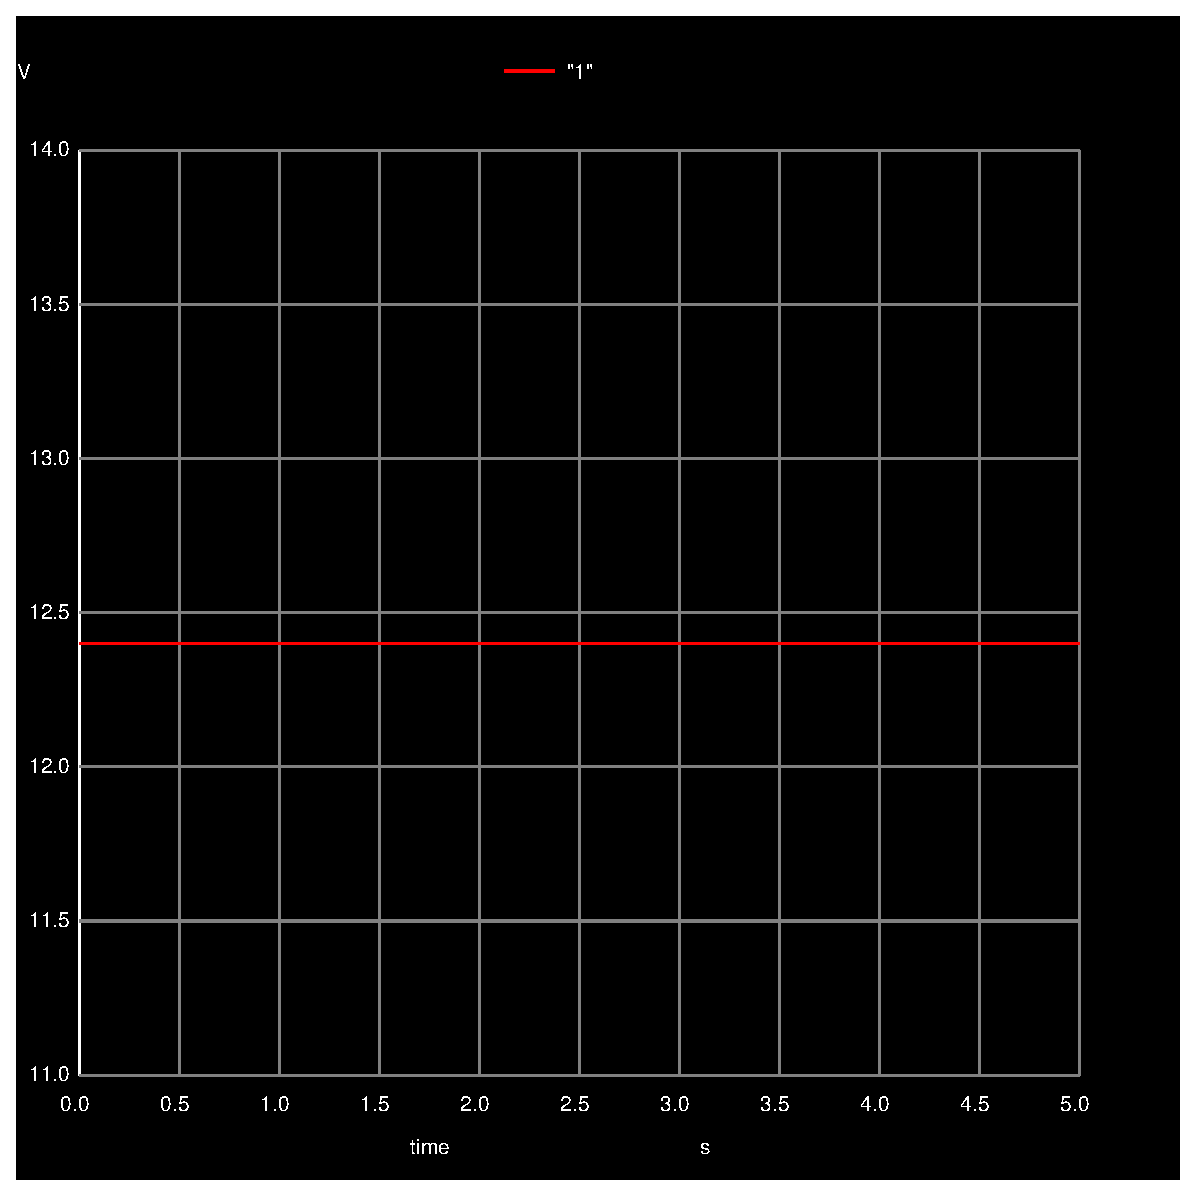
\includegraphics[width=6.5cm]{011.ps}
 \caption{R1}
 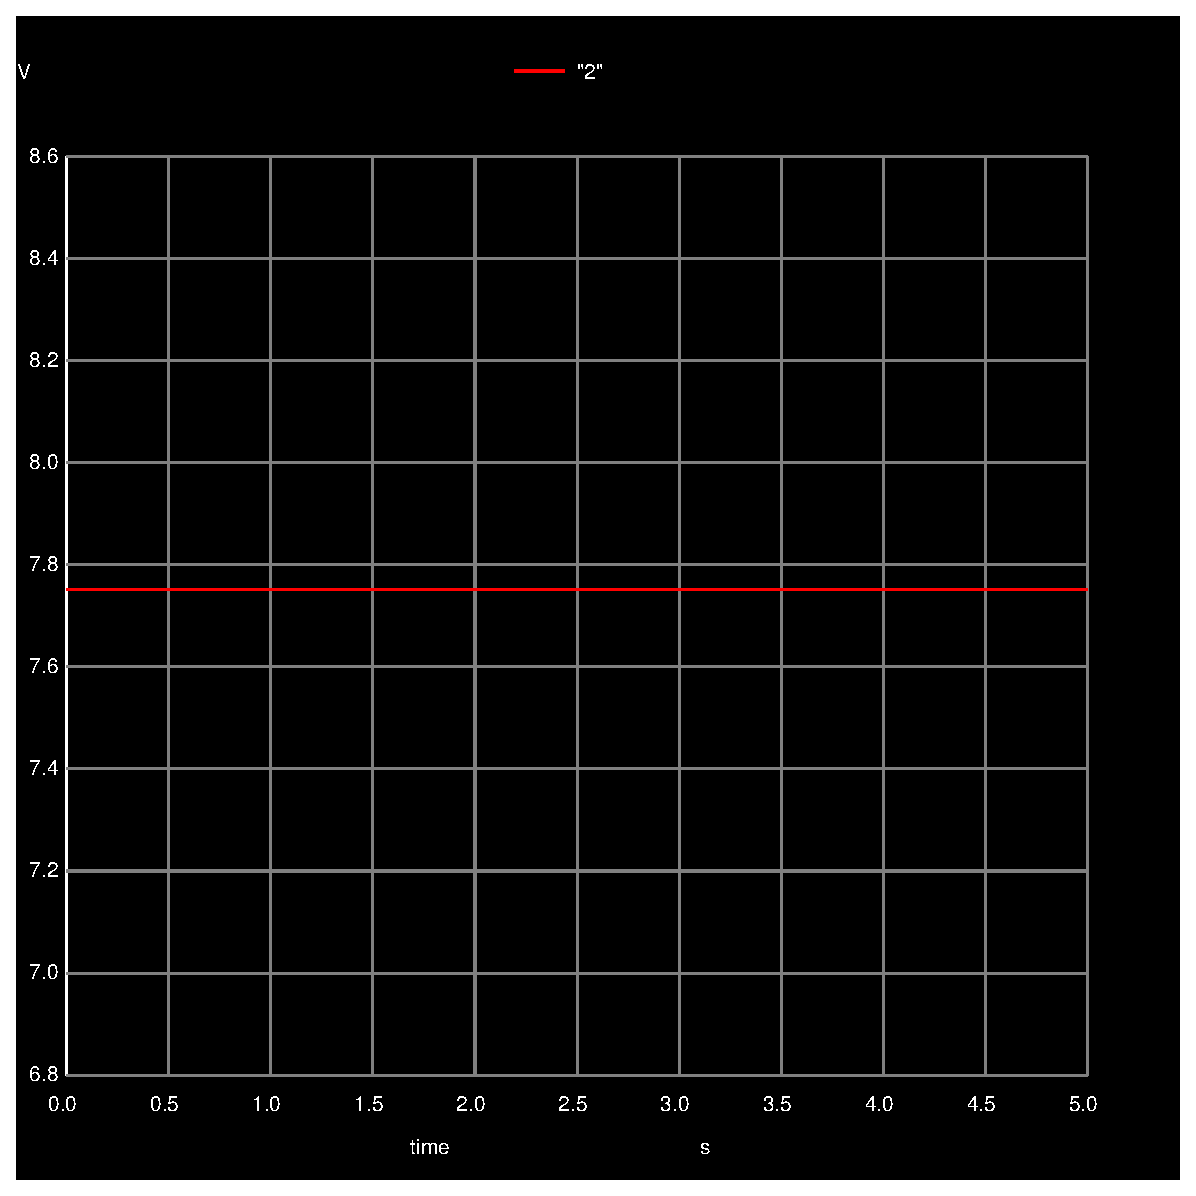
\includegraphics[width=6.5cm]{012.ps}
  \caption{R2}
  \label{2}
\end{figure}

\newpage
\section{Darbs ar QUCS programmām}
\begin{figure}[h]
    \centering
\rotatebox{-90}{\includegraphics[trim=0 0 265 200, width=12cm]{print.ps}}
    \caption{DC simulation}
    \label{3}
\end{figure}
1. attēlā jūs varat redzēt visas komponentes savienotas vienā ķēdē. \ 
2. attēlā(augšējais pa labi) jūs varat redzēt 'Parameter sweep' kurā var redzēt atribūtus un to parametrus. \
3. attēlā var redzēt tabulu ar visiem parametriem. \ 
4 attēlā var redzēt grafiku. \ 


\begin{thebibliography}{9}
\bibitem{1.}
Albert Einstein. 
\textit{Zur Elektrodynamik bewegter K{\"o}rper}. (German) 
[\textit{On the electrodynamics of moving bodies}]
Annalen der Physik, 322(10):891–921, 1905.

\bibitem{2.} 
Michel Goossens, Frank Mittelbach, and Alexander Samarin. 
\textit{The \LaTeX\ Companion}. 
Addison-Wesley, Reading, Massachusetts, 1993.
\end{thebibliography}


\end{document}